\documentclass{report}

%%%%%%%%%%%%%%%%%%%%%%%%%%%%%%%%%
% PACKAGE IMPORTS
%%%%%%%%%%%%%%%%%%%%%%%%%%%%%%%%%

\usepackage[utf8]{inputenc} % Сурс - семинары по алгебре Медведя Никиты Юрьевича
\usepackage[T2A]{fontenc}

\usepackage[tmargin=2cm,rmargin=1in,lmargin=1in,margin=0.85in,bmargin=2cm,footskip=.2in]{geometry}
\usepackage{amsmath,amsfonts,amsthm,amssymb,mathtools}
\usepackage[varbb]{newpxmath}
\usepackage{xfrac}
\usepackage[makeroom]{cancel}
\usepackage{mathtools}
\usepackage{bookmark}
\usepackage{enumitem}
\usepackage{hyperref,theoremref}
\hypersetup{
	pdftitle={Assignment},
	colorlinks=true, linkcolor=doc!90,
	bookmarksnumbered=true,
	bookmarksopen=true
}
\usepackage[most,many,breakable]{tcolorbox}
\usepackage{xcolor}% http://ctan.org/pkg/xcolor
%\usepackage{colortbl}% http://ctan.org/pkg/colortbl
\usepackage{multirow}% http://ctan.org/pkg/multirow
\usepackage{graphicx}% http://ctan.org/pkg/graphicx
\usepackage{varwidth}
\usepackage{varwidth}
\usepackage{etoolbox}
\usepackage{anyfontsize}
% \usepackage{lmodern}
%\usepackage{authblk}
\usepackage{nameref}
\usepackage{multicol,array}
\usepackage{tikz-cd}
\usepackage[ruled,vlined,linesnumbered]{algorithm2e}
\usepackage{comment} % enables the use of multi-line comments (\ifx \fi) 
\usepackage{import}
\usepackage{xifthen}
\usepackage{pdfpages}
\usepackage{transparent}

\usepackage[english]{babel}
% ,russian
\usepackage{amsfonts,amssymb}
\usepackage{relsize}

\usepackage{systeme}

\usepackage{indentfirst} % Красная строка
\usepackage{fancyhdr}
\usepackage{wrapfig}
\usepackage{textcomp}

\usepackage{physics}

% \usepackage[unicode]{hyperref}

\newcommand\mycommfont[1]{\footnotesize\ttfamily\textcolor{blue}{#1}}
\SetCommentSty{mycommfont}
\newcommand{\incfig}[1]{%
    \def\svgwidth{\columnwidth}
    \import{./figures/}{#1.pdf_tex}
}

\usepackage{tikzsymbols}
\renewcommand\qedsymbol{$\blacksquare$}

\usepackage{sectsty}

% strikethrough text \sout
\usepackage[normalem]{ulem}

\usepackage{code}

\chapternumberfont{\normalsize} 
\chaptertitlefont{\Large}
% \fontsize{<size>}{<line space>}
\sectionfont{\fontsize{12}{15}\selectfont}

% <chapter>.<section> -> <section> indexing in report mode
% \renewcommand{\thesection}{\arabic{section}}

%\usepackage{import}
%\usepackage{xifthen}
%\usepackage{pdfpages}
%\usepackage{transparent}


%%%%%%%%%%%%%%%%%%%%%%%%%%%%%%
% SELF MADE COLORS
%%%%%%%%%%%%%%%%%%%%%%%%%%%%%%



\definecolor{myg}{RGB}{56, 140, 70}
\definecolor{myb}{RGB}{45, 111, 177}
\definecolor{myr}{RGB}{199, 68, 64}
\definecolor{mytheorembg}{HTML}{F2F2F9}
\definecolor{mytheoremfr}{HTML}{00007B}
\definecolor{mylemmabg}{HTML}{FFFAF8}
\definecolor{mylemmafr}{HTML}{983b0f}
\definecolor{mypropbg}{HTML}{f2fbfc}
\definecolor{mypropfr}{HTML}{191971}
\definecolor{myexamplebg}{HTML}{F2FBF8}
\definecolor{myexamplefr}{HTML}{88D6D1}
\definecolor{myexampleti}{HTML}{2A7F7F}
\definecolor{mydefinitbg}{HTML}{E5E5FF}
\definecolor{mydefinitfr}{HTML}{3F3FA3}
\definecolor{notesgreen}{RGB}{0,162,0}
\definecolor{myp}{RGB}{197, 92, 212}
\definecolor{mygr}{HTML}{2C3338}
\definecolor{myred}{RGB}{127,0,0}
\definecolor{myyellow}{RGB}{169,121,69}
\definecolor{myexercisebg}{HTML}{F2FBF8}
\definecolor{myexercisefg}{HTML}{88D6D1}

\definecolor{myclarificationbg}{HTML}{FFFAF8}
\definecolor{myclarificationfr}{HTML}{983b0f}


%%%%%%%%%%%%%%%%%%%%%%%%%%%%
% TCOLORBOX SETUPS
%%%%%%%%%%%%%%%%%%%%%%%%%%%%

\setlength{\parindent}{1cm}
%================================
% THEOREM BOX
%================================

\tcbuselibrary{theorems,skins,hooks}
\newtcbtheorem[number within=section]{Theorem}{Theorem}
{%
	enhanced,
	breakable,
	colback = mytheorembg,
	frame hidden,
	boxrule = 0sp,
	borderline west = {2pt}{0pt}{mytheoremfr},
	sharp corners,
	detach title,
	before upper = \tcbtitle\par\smallskip,
	coltitle = mytheoremfr,
	fonttitle = \bfseries\sffamily,
	description font = \mdseries,
	separator sign none,
	segmentation style={solid, mytheoremfr},
}
{th}

\tcbuselibrary{theorems,skins,hooks}
\newtcbtheorem[number within=chapter]{theorem}{Theorem}
{%
	enhanced,
	% breakable,
	colback = mytheorembg,
	frame hidden,
	boxrule = 0sp,
	borderline west = {2pt}{0pt}{mytheoremfr},
	sharp corners,
	detach title,
	before upper = \tcbtitle\par\smallskip,
	coltitle = mytheoremfr,
	fonttitle = \bfseries\sffamily,
	description font = \mdseries,
	separator sign none,
	segmentation style={solid, mytheoremfr},
}
{th}


\tcbuselibrary{theorems,skins,hooks}
\newtcolorbox{Theoremcon}
{%
	enhanced
	,breakable
	,colback = mytheorembg
	,frame hidden
	,boxrule = 0sp
	,borderline west = {2pt}{0pt}{mytheoremfr}
	,sharp corners
	,description font = \mdseries
	,separator sign none
}

%================================
% Corollery
%================================
\tcbuselibrary{theorems,skins,hooks}
\newtcbtheorem[number within=section]{Corollary}{Corollary}
{%
	enhanced
	,breakable
	,colback = myp!10
	,frame hidden
	,boxrule = 0sp
	,borderline west = {2pt}{0pt}{myp!85!black}
	,sharp corners
	,detach title
	,before upper = \tcbtitle\par\smallskip
	,coltitle = myp!85!black
	,fonttitle = \bfseries\sffamily
	,description font = \mdseries
	,separator sign none
	,segmentation style={solid, myp!85!black}
}
{th}
\tcbuselibrary{theorems,skins,hooks}
\newtcbtheorem[number within=chapter]{corollary}{Corollary}
{%
	enhanced,
	% breakable,
	colback = myp!10,
	frame hidden,
	boxrule = 0sp,
	borderline west = {2pt}{0pt}{myp!85!black},
	sharp corners,
	detach title,
	before upper = \tcbtitle\par\smallskip,
	coltitle = myp!85!black,
	fonttitle = \bfseries\sffamily,
	description font = \mdseries,
	separator sign none,
	segmentation style={solid, myp!85!black}
}
{th}


%================================
% LENMA
%================================

\tcbuselibrary{theorems,skins,hooks}
\newtcbtheorem[number within=section]{Lemma}{Lemma}
{%
	enhanced,
	breakable,
	colback = mylemmabg,
	frame hidden,
	boxrule = 0sp,
	borderline west = {2pt}{0pt}{mylemmafr},
	sharp corners,
	detach title,
	before upper = \tcbtitle\par\smallskip,
	coltitle = mylemmafr,
	fonttitle = \bfseries\sffamily,
	description font = \mdseries,
	separator sign none,
	segmentation style={solid, mylemmafr},
}
{th}

\tcbuselibrary{theorems,skins,hooks}
\newtcbtheorem[number within=chapter]{lemma}{Lemma}
{%
	enhanced,
	% breakable,
	colback = mylemmabg,
	frame hidden,
	boxrule = 0sp,
	borderline west = {2pt}{0pt}{mylemmafr},
	sharp corners,
	detach title,
	before upper = \tcbtitle\par\smallskip,
	coltitle = mylemmafr,
	fonttitle = \bfseries\sffamily,
	description font = \mdseries,
	separator sign none,
	segmentation style={solid, mylemmafr},
}
{th}


%================================
% PROPOSITION
%================================

\tcbuselibrary{theorems,skins,hooks}
\newtcbtheorem[number within=section]{Prop}{Proposition}
{%
	enhanced,
	breakable,
	colback = mypropbg,
	frame hidden,
	boxrule = 0sp,
	borderline west = {2pt}{0pt}{mypropfr},
	sharp corners,
	detach title,
	before upper = \tcbtitle\par\smallskip,
	coltitle = mypropfr,
	fonttitle = \bfseries\sffamily,
	description font = \mdseries,
	separator sign none,
	segmentation style={solid, mypropfr},
}
{th}

\tcbuselibrary{theorems,skins,hooks}
\newtcbtheorem[number within=chapter]{prop}{Proposition}
{%
	enhanced,
	% breakable,
	colback = mypropbg,
	frame hidden,
	boxrule = 0sp,
	borderline west = {2pt}{0pt}{mypropfr},
	sharp corners,
	detach title,
	before upper = \tcbtitle\par\smallskip,
	coltitle = mypropfr,
	fonttitle = \bfseries\sffamily,
	description font = \mdseries,
	separator sign none,
	segmentation style={solid, mypropfr},
}
{th}


%================================
% CLAIM
%================================

\tcbuselibrary{theorems,skins,hooks}
\newtcbtheorem[number within=section]{Claim}{Claim}
{%
	enhanced,
	breakable,
	colback = myg!10,
	frame hidden,
	boxrule = 0sp,
	borderline west = {2pt}{0pt}{myg},
	sharp corners,
	detach title,
	before upper = \tcbtitle\par\smallskip,
	coltitle = myg!85!black,
	fonttitle = \bfseries\sffamily,
	description font = \mdseries,
	separator sign none,
	segmentation style={solid, myg!85!black}
}
{th}

\tcbuselibrary{theorems,skins,hooks}
\newtcbtheorem[number within=section]{claim}{Claim}
{%
	enhanced,
	% breakable,
	colback = myg!10,
	frame hidden,
	boxrule = 0sp,
	borderline west = {2pt}{0pt}{myg},
	sharp corners,
	detach title,
	before upper = \tcbtitle\par\smallskip,
	coltitle = myg!85!black,
	fonttitle = \bfseries\sffamily,
	description font = \mdseries,
	separator sign none,
	segmentation style={solid, myg!85!black}
}
{th}


%================================
% Exercise
%================================

\tcbuselibrary{theorems,skins,hooks}
\newtcbtheorem[number within=section]{Exercise}{Exercise}
{%
	enhanced,
	breakable,
	colback = myexercisebg,
	frame hidden,
	boxrule = 0sp,
	borderline west = {2pt}{0pt}{myexercisefg},
	sharp corners,
	detach title,
	before upper = \tcbtitle\par\smallskip,
	coltitle = myexercisefg,
	fonttitle = \bfseries\sffamily,
	description font = \mdseries,
	separator sign none,
	segmentation style={solid, myexercisefg},
}
{th}

\tcbuselibrary{theorems,skins,hooks}
\newtcbtheorem[number within=chapter]{exercise}{Exercise}
{%
	enhanced,
	% breakable,
	colback = myexercisebg,
	frame hidden,
	boxrule = 0sp,
	borderline west = {2pt}{0pt}{myexercisefg},
	sharp corners,
	detach title,
	before upper = \tcbtitle\par\smallskip,
	coltitle = myexercisefg,
	fonttitle = \bfseries\sffamily,
	description font = \mdseries,
	separator sign none,
	segmentation style={solid, myexercisefg},
}
{th}

%================================
% EXAMPLE BOX
%================================

\newtcbtheorem[number within=section]{Example}{Example}
{%
	colback = myexamplebg,
	breakable,
	colframe = myexamplefr,
	coltitle = myexampleti,
	boxrule = 1pt,
	sharp corners,
	detach title,
	before upper=\tcbtitle\par\smallskip,
	fonttitle = \bfseries,
	description font = \mdseries,
	separator sign none,
	description delimiters parenthesis
}
{ex}

\newtcbtheorem[number within=chapter]{example}{Example}
{%
	colback = myexamplebg,
	% breakable,
	colframe = myexamplefr,
	coltitle = myexampleti,
	boxrule = 1pt,
	sharp corners,
	detach title,
	before upper=\tcbtitle\par\smallskip,
	fonttitle = \bfseries,
	description font = \mdseries,
	separator sign none,
	description delimiters parenthesis
}
{ex}

%================================
% DEFINITION BOX
%================================

\newtcbtheorem[number within=section]{Definition}{Definition}{enhanced,
	before skip=2mm,after skip=2mm, colback=red!5,colframe=red!80!black,boxrule=0.5mm,
	attach boxed title to top left={xshift=1cm,yshift*=1mm-\tcboxedtitleheight}, varwidth boxed title*=-3cm,
	boxed title style={frame code={
					\path[fill=tcbcolback]
					([yshift=-1mm,xshift=-1mm]frame.north west)
					arc[start angle=0,end angle=180,radius=1mm]
					([yshift=-1mm,xshift=1mm]frame.north east)
					arc[start angle=180,end angle=0,radius=1mm];
					\path[left color=tcbcolback!60!black,right color=tcbcolback!60!black,
						middle color=tcbcolback!80!black]
					([xshift=-2mm]frame.north west) -- ([xshift=2mm]frame.north east)
					[rounded corners=1mm]-- ([xshift=1mm,yshift=-1mm]frame.north east)
					-- (frame.south east) -- (frame.south west)
					-- ([xshift=-1mm,yshift=-1mm]frame.north west)
					[sharp corners]-- cycle;
				},interior engine=empty,
		},
	fonttitle=\bfseries,
	title={#2},#1}{def}
\newtcbtheorem[number within=chapter]{definition}{Definition}{enhanced,
	before skip=2mm,after skip=2mm, colback=red!5,colframe=red!80!black,boxrule=0.5mm,
	attach boxed title to top left={xshift=1cm,yshift*=1mm-\tcboxedtitleheight}, varwidth boxed title*=-3cm,
	boxed title style={frame code={
					\path[fill=tcbcolback]
					([yshift=-1mm,xshift=-1mm]frame.north west)
					arc[start angle=0,end angle=180,radius=1mm]
					([yshift=-1mm,xshift=1mm]frame.north east)
					arc[start angle=180,end angle=0,radius=1mm];
					\path[left color=tcbcolback!60!black,right color=tcbcolback!60!black,
						middle color=tcbcolback!80!black]
					([xshift=-2mm]frame.north west) -- ([xshift=2mm]frame.north east)
					[rounded corners=1mm]-- ([xshift=1mm,yshift=-1mm]frame.north east)
					-- (frame.south east) -- (frame.south west)
					-- ([xshift=-1mm,yshift=-1mm]frame.north west)
					[sharp corners]-- cycle;
				},interior engine=empty,
		},
	fonttitle=\bfseries,
	title={#2},#1}{def}



%================================
% Solution BOX
%================================

\makeatletter
\newtcolorbox{solution}{enhanced,
	breakable,
	colback=white,
	colframe=myg!80!black,
	attach boxed title to top left={yshift*=-\tcboxedtitleheight},
	title=Solution,
	boxed title size=title,
	boxed title style={%
			sharp corners,
			rounded corners=northwest,
			colback=tcbcolframe,
			boxrule=0pt,
		},
	underlay boxed title={%
			\path[fill=tcbcolframe] (title.south west)--(title.south east)
			to[out=0, in=180] ([xshift=5mm]title.east)--
			(title.center-|frame.east)
			[rounded corners=\kvtcb@arc] |-
			(frame.north) -| cycle;
		},
}
\makeatother

%================================
% Question BOX
%================================

\makeatletter
\newtcbtheorem{Question}{Question}{enhanced,
	breakable,
	colback=white,
	colframe=mygr,
	attach boxed title to top left={yshift*=-\tcboxedtitleheight},
	fonttitle=\bfseries,
	title={#2},
	boxed title size=title,
	boxed title style={%
			sharp corners,
			rounded corners=northwest,
			colback=tcbcolframe,
			boxrule=0pt,
		},
	underlay boxed title={%
			\path[fill=tcbcolframe] (title.south west)--(title.south east)
			to[out=0, in=180] ([xshift=5mm]title.east)--
			(title.center-|frame.east)
			[rounded corners=\kvtcb@arc] |-
			(frame.north) -| cycle;
		},
	#1
}{def}
\makeatother

\makeatletter
\newtcbtheorem{question}{Question}{enhanced,
	% breakable,
	colback=white,
	colframe=mygr,
	attach boxed title to top left={yshift*=-\tcboxedtitleheight},
	fonttitle=\bfseries,
	title={#2},
	boxed title size=title,
	boxed title style={%
			sharp corners,
			rounded corners=northwest,
			colback=tcbcolframe,
			boxrule=0pt,
		},
	underlay boxed title={%
			\path[fill=tcbcolframe] (title.south west)--(title.south east)
			to[out=0, in=180] ([xshift=5mm]title.east)--
			(title.center-|frame.east)
			[rounded corners=\kvtcb@arc] |-
			(frame.north) -| cycle;
		},
	#1
}{def}
\makeatother

\newtcbtheorem[number within=chapter]{wconc}{Wrong Concept}{
	breakable,
	enhanced,
	colback=white,
	colframe=myr,
	arc=0pt,
	outer arc=0pt,
	fonttitle=\bfseries\sffamily\large,
	colbacktitle=myr,
	attach boxed title to top left={},
	boxed title style={
			enhanced,
			skin=enhancedfirst jigsaw,
			arc=3pt,
			bottom=0pt,
			interior style={fill=myr}
		},
	#1
}{def}



%================================
% NOTE BOX
%================================

\usetikzlibrary{arrows,calc,shadows.blur}
\tcbuselibrary{skins}
\newtcolorbox{note}[1][]{%
	enhanced jigsaw,
	colback=gray!20!white,%
	colframe=gray!80!black,
	size=small,
	boxrule=1pt,
	title=\textbf{Note},
	halign title=flush center,
	coltitle=black,
	breakable,
	drop shadow=black!50!white,
	attach boxed title to top left={xshift=1cm,yshift=-\tcboxedtitleheight/2,yshifttext=-\tcboxedtitleheight/2},
	minipage boxed title=1.5cm,
	boxed title style={%
			colback=white,
			size=fbox,
			boxrule=1pt,
			boxsep=2pt,
			underlay={%
					\coordinate (dotA) at ($(interior.west) + (-0.5pt,0)$);
					\coordinate (dotB) at ($(interior.east) + (0.5pt,0)$);
					\begin{scope}
						\clip (interior.north west) rectangle ([xshift=3ex]interior.east);
						\filldraw [white, blur shadow={shadow opacity=60, shadow yshift=-.75ex}, rounded corners=2pt] (interior.north west) rectangle (interior.south east);
					\end{scope}
					\begin{scope}[gray!80!black]
						\fill (dotA) circle (2pt);
						\fill (dotB) circle (2pt);
					\end{scope}
				},
		},
	#1,
}

%================================
% Clarification box
%================================

\newtcbtheorem[number within=section]{Clarification}{Clarification}
{%
	colback = myclarificationbg,
	breakable,
	colframe = myclarificationfr,
	coltitle = myexampleti,
	boxrule = 1pt,
	sharp corners,
	detach title,
	before upper=\tcbtitle\par\smallskip,
	fonttitle = \bfseries,
	description font = \mdseries,
	separator sign none,
	description delimiters parenthesis
}
{clarif}

\newtcbtheorem[number within=chapter]{clarification}{Clarification}
{%
	colback = myclarificationbg,
	% breakable,
	colframe = myclarificationfr,
	coltitle = myexampleti,
	boxrule = 1pt,
	sharp corners,
	detach title,
	before upper=\tcbtitle\par\smallskip,
	fonttitle = \bfseries,
	description font = \mdseries,
	separator sign none,
	description delimiters
}
{clarif}

%%%%%%%%%%%%%%%%%%%%%%%%%%%%%%
% SELF MADE COMMANDS
%%%%%%%%%%%%%%%%%%%%%%%%%%%%%%

\newcommand{\nt}[1]{\begin{note}#1\end{note}}

\newcommand{\mcthmBreakable}[2]{\begin{Theorem*}{#1}{}#2\end{Theorem*}}
\newcommand{\mcthm}[2]{\begin{theorem*}{#1}{}#2\end{theorem*}}
\newcommand{\mccorollarBreakable}[2]{\begin{Corollary*}{#1}{}#2\end{Corollary*}}
\newcommand{\mccorollar}[2]{\begin{corollary*}{#1}{}#2\end{corollary*}}
\newcommand{\mcpropBreakable}[2]{\begin{Prop*}{#1}{}#2\end{Prop*}}
\newcommand{\mcprop}[2]{\begin{prop*}{#1}{}#2\end{prop*}}
\newcommand{\mcdfnBreakable}[2]{\begin{Definition*}[colbacktitle=red!75!black]{#1}{}#2\end{Definition*}}
\newcommand{\mcdfn}[2]{\begin{definition*}[colbacktitle=red!75!black]{#1}{}#2\end{definition*}}
\newcommand{\mcexBreakable}[2]{\begin{Example*}{#1}{}#2\end{Example*}}
\newcommand{\mcex}[2]{\begin{example*}{#1}{}#2\end{example*}}
\newcommand{\mcprf}[1]{\begin{mcproof}\[#1\]\end{mcproof}}
\newcommand{\mcproofpure}[1]{\begin{mcproof}#1\end{mcproof}}
\newcommand{\mcclmBreakable}[3]{\begin{Claim*}{#1}{#2}#3\end{Claim*}}
\newcommand{\mcclm}[3]{\begin{claim*}{#1}{#2}#3\end{claim*}}
\newcommand{\mcclarfBreakable}[2]{\begin{Clarification*}{#1}{}#2\end{Clarification*}}
\newcommand{\mcclarf}[2]{\begin{clarification*}{#1}{}#2\end{clarification*}}
\newcommand{\mclemmaBreakable}[2]{\begin{Lemma*}{#1}{}#2\end{Lemma*}}
\newcommand{\mclemma}[2]{\begin{lemma*}{#1}{}#2\end{lemma*}}

\newenvironment{myclaim}[1][\claimname]{\proof[\bfseries #1: ]}{}

\newcommand*\circled[1]{\tikz[baseline=(char.base)]{
		\node[shape=circle,draw,inner sep=1pt] (char) {#1};}}
\newcommand\getcurrentref[1]{%
	\ifnumequal{\value{#1}}{0}
	{??}
	{\the\value{#1}}%
}
\newcommand{\getCurrentSectionNumber}{\getcurrentref{section}}
\newenvironment{mcproof}[1][\proofname]{%
	\proof[\bfseries #1: ]%
}{\endproof}


\newcounter{mylabelcounter}

\makeatletter
\newcommand{\setword}[2]{%
	\phantomsection
	#1\def\@currentlabel{\unexpanded{#1}}\label{#2}%
}
\makeatother


\tikzset{
	symbol/.style={
			draw=none,
			every to/.append style={
					edge node={node [sloped, allow upside down, auto=false]{$#1$}}}
		}
}


% deliminators
% \DeclarePairedDelimiter{\abs}{\lvert}{\rvert}  % declared in <physics>
% \DeclarePairedDelimiter{\norm}{\lVert}{\rVert} % declared in <physics>

\DeclarePairedDelimiter{\ceil}{\lceil}{\rceil}
\DeclarePairedDelimiter{\floor}{\lfloor}{\rfloor}
\DeclarePairedDelimiter{\round}{\lfloor}{\rceil}

\newsavebox\diffdbox
\newcommand{\slantedromand}{{\mathpalette\makesl{d}}}
\newcommand{\makesl}[2]{%
\begingroup
\sbox{\diffdbox}{$\mathsurround=0pt#1\mathrm{#2}$}%
\pdfsave
\pdfsetmatrix{1 0 0.2 1}%
\rlap{\usebox{\diffdbox}}%
\pdfrestore
\hskip\wd\diffdbox
\endgroup
}
\newcommand{\mcdd}[1][]{\ensuremath{\mathop{}\!\ifstrempty{#1}{%
\slantedromand\@ifnextchar^{\hspace{0.2ex}}{\hspace{0.1ex}}}%
{\slantedromand\hspace{0.2ex}^{#1}}}}
\ProvideDocumentCommand\dv{o m g}{%
  \ensuremath{%
    \IfValueTF{#3}{%
      \IfNoValueTF{#1}{%
        \frac{\mcdd #2}{\mcdd #3}%
      }{%
        \frac{\mcdd^{#1} #2}{\mcdd #3^{#1}}%
      }%
    }{%
      \IfNoValueTF{#1}{%
        \frac{\mcdd}{\mcdd #2}%
      }{%
        \frac{\mcdd^{#1}}{\mcdd #2^{#1}}%
      }%
    }%
  }%
}
\providecommand*{\pdv}[3][]{\frac{\partial^{#1}#2}{\partial#3^{#1}}}

% Since the amsthm package isn't loaded

% I prefer the slanted \leq
\let\oldleq\leq % save them in case they're every wanted
\let\oldgeq\geq
\renewcommand{\leq}{\leqslant}
\renewcommand{\geq}{\geqslant}

% % redefine matrix env to allow for alignment, use r as default
% \renewcommand*\env@matrix[1][r]{\hskip -\arraycolsep
%     \let\@ifnextchar\new@ifnextchar
%     \array{*\c@MaxMatrixCols #1}}


%\usepackage{framed}
%\usepackage{titletoc}
%\usepackage{etoolbox}
%\usepackage{lmodern}


%\patchcmd{\tableofcontents}{\contentsname}{\sffamily\contentsname}{}{}

%\renewenvironment{leftbar}
%{\def\FrameCommand{\hspace{6em}%
%		{\color{myyellow}\vrule width 2pt depth 6pt}\hspace{1em}}%
%	\MakeFramed{\parshape 1 0cm \dimexpr\textwidth-6em\relax\FrameRestore}\vskip2pt%
%}
%{\endMakeFramed}

%\titlecontents{chapter}
%[0em]{\vspace*{2\baselineskip}}
%{\parbox{4.5em}{%
%		\hfill\Huge\sffamily\bfseries\color{myred}\thecontentspage}%
%	\vspace*{-2.3\baselineskip}\leftbar\textsc{\small\chaptername~\thecontentslabel}\\\sffamily}
%{}{\endleftbar}
%\titlecontents{section}
%[8.4em]
%{\sffamily\contentslabel{3em}}{}{}
%{\hspace{0.5em}\nobreak\itshape\color{myred}\contentspage}
%\titlecontents{subsection}
%[8.4em]
%{\sffamily\contentslabel{3em}}{}{}  
%{\hspace{0.5em}\nobreak\itshape\color{myred}\contentspage}


%%%%%%%%%%%%%%%%%%%%%%%%%%%%%%%%%%%%%%%%%%%
% TABLE OF CONTENTS
%%%%%%%%%%%%%%%%%%%%%%%%%%%%%%%%%%%%%%%%%%%

\usepackage{tikz}
\definecolor{doc}{RGB}{0,60,110}
\usepackage{titletoc}

% \contentsmargin{0cm}
% \titlecontents{chapter}[3.7pc]
% {\addvspace{30pt}%
% 	\begin{tikzpicture}[remember picture, overlay]%
% 		\draw[fill=doc!60,draw=doc!60] (-7,-.1) rectangle (-0.9,.5);%
% 		\pgftext[left,x=-3.5cm,y=0.2cm]{\color{white}\Large\sc\bfseries Chapter\ \thecontentslabel};%
% 	\end{tikzpicture}\color{doc!60}\large\sc\bfseries}%
% {}
% {}
% {\;\titlerule\;\large\sc\bfseries Page \thecontentspage
% 	\begin{tikzpicture}[remember picture, overlay]
% 		\draw[fill=doc!60,draw=doc!60] (2pt,0) rectangle (4,0.1pt);
% 	\end{tikzpicture}}%
% \titlecontents{section}[3.7pc]
% {\addvspace{2pt}}
% {\contentslabel[\thecontentslabel]{2pc}}
% {}
% {\hfill\small \thecontentspage}
% []
% \titlecontents*{subsection}[3.7pc]
% {\addvspace{-1pt}\small}
% {}
% {}
% {\ --- \small\thecontentspage}
% [ \textbullet\ ][]

% \makeatletter
% \renewcommand{\tableofcontents}{%
% 	\chapter*{%
% 	  \vspace*{-20\p@}%
% 	  \begin{tikzpicture}[remember picture, overlay]%
% 		  \pgftext[right,x=15cm,y=0.2cm]{\color{doc!60}\Huge\sc\bfseries \contentsname};%
% 		  \draw[fill=doc!60,draw=doc!60] (13,-.75) rectangle (20,1);%
% 		  \clip (13,-.75) rectangle (20,1);
% 		  \pgftext[right,x=15cm,y=0.2cm]{\color{white}\Huge\sc\bfseries \contentsname};%
% 	  \end{tikzpicture}}%
% 	\@starttoc{toc}}
% \makeatother


%From M275 "Topology" at SJSU
\newcommand{\id}{\mathrm{id}}
\newcommand{\taking}[1]{\xrightarrow{#1}}
\newcommand{\inv}{^{-1}}

%From M170 "Introduction to Graph Theory" at SJSU
\DeclareMathOperator{\diam}{diam}
\DeclareMathOperator{\ord}{ord}
\newcommand{\defeq}{\overset{\mathrm{def}}{=}}

%From the USAMO .tex files
\newcommand{\ts}{\textsuperscript}
\newcommand{\dg}{^\circ}
\newcommand{\ii}{\item}

% % From Math 55 and Math 145 at Harvard
% \newenvironment{subproof}[1][Proof]{%
% \begin{proof}[#1] \renewcommand{\qedsymbol}{$\blacksquare$}}%
% {\end{proof}}

\newcommand{\liff}{\leftrightarrow}
\newcommand{\lthen}{\rightarrow}
\newcommand{\opname}{\operatorname}
\newcommand{\surjto}{\twoheadrightarrow}
\newcommand{\injto}{\hookrightarrow}
\newcommand{\On}{\mathrm{On}}        % ordinals
\DeclareMathOperator{\img}{im}       % Image
\DeclareMathOperator{\Img}{Im}       % Image
\DeclareMathOperator{\coker}{coker}  % Cokernel
\DeclareMathOperator{\Coker}{Coker}  % Cokernel
\DeclareMathOperator{\Ker}{Ker}      % Kernel
% \DeclareMathOperator{\rank}{rank}  % rank       % declared in <physics>
\DeclareMathOperator{\Spec}{Spec}    % spectrum
% \DeclareMathOperator{\Tr}{Tr}      % trace      % declared in <physics>
\DeclareMathOperator{\pr}{pr}        % projection
\DeclareMathOperator{\ext}{ext}      % extension
\DeclareMathOperator{\pred}{pred}    % predecessor
\DeclareMathOperator{\dom}{dom}      % domain
\DeclareMathOperator{\ran}{ran}      % range
\DeclareMathOperator{\Hom}{Hom}      % homomorphism
\DeclareMathOperator{\Mor}{Mor}      % morphisms
\DeclareMathOperator{\End}{End}      % endomorphism

\DeclareMathOperator{\lowlim}{\underline{lim}} % lower limit
\DeclareMathOperator{\uplim}{\overline{lim}}   % upper limit

% combinations
\newcommand{\Cmb}[2]{ C^{#2}_{#1} }
\newcommand{\NumSeq}[1]{\{ #1 \}}
\newcommand{\SmO}[1][x]{\overline{o}(#1)}

%probabilities
\newcommand{\Proba}[1]{\mathds{P}\left( #1 \right)}
\newcommand{\Probc}[2]{\mathds{P}\left( #1 ~\vert~ #2\right)}

%expected values
\newcommand{\E}[1]{\mathds{E} \left( #1 \right) }
\newcommand{\Ec}[2]{\mathds{E} \left[ #1 ~\vert ~ #2\right] }

% - others
\DeclareMathOperator{\Lap}{\mathcal{L}}
\DeclareMathOperator{\Var}{var} % varience
\DeclareMathOperator{\cov}{cov} % covarience

\newcommand{\veps}{\varepsilon}
\newcommand{\wt}{\widetilde}
\newcommand{\wh}{\widehat}
\newcommand{\vocab}[1]{\textbf{\color{blue} #1}}
\providecommand{\half}{\frac{1}{2}}
\newcommand{\dang}{\measuredangle} %% Directed angle
\newcommand{\ray}[1]{\overrightarrow{#1}}
\newcommand{\seg}[1]{\overline{#1}}
\newcommand{\arc}[1]{\wideparen{#1}}
\DeclareMathOperator{\cis}{cis}
\DeclareMathOperator*{\lcm}{lcm}

\DeclareMathOperator*{\argmin}{arg min}
\DeclareMathOperator*{\argmax}{arg max}

% Contradiction symbol (like \bot)
\newcommand{\Contradiction}{\ensuremath{\circled{$\mathbb{W}$}}}

\newcommand{\cycsum}{\sum_{\mathrm{cyc}}}
\newcommand{\symsum}{\sum_{\mathrm{sym}}}
\newcommand{\cycprod}{\prod_{\mathrm{cyc}}}
\newcommand{\symprod}{\prod_{\mathrm{sym}}}
\newcommand{\Qed}{\begin{flushright}\qed\end{flushright}}
\newcommand{\parinn}{\setlength{\parindent}{1cm}}
\newcommand{\parinf}{\setlength{\parindent}{0cm}}
% \newcommand{\norm}{\|\cdot\|}                         % declared in <physics>
\newcommand{\inorm}{\norm_{\infty}}
\newcommand{\opensets}{\{V_{\alpha}\}_{\alpha\in I}}
\newcommand{\oset}{V_{\alpha}}
\newcommand{\opset}[1]{V_{\alpha_{#1}}}
\newcommand{\lub}{\text{lub}}
\newcommand{\del}[2]{\frac{\partial #1}{\partial #2}}
\newcommand{\Del}[3]{\frac{\partial^{#1} #2}{\partial^{#1} #3}}
\newcommand{\deld}[2]{\dfrac{\partial #1}{\partial #2}}
\newcommand{\Deld}[3]{\dfrac{\partial^{#1} #2}{\partial^{#1} #3}}
\newcommand{\lm}{\lambda}
\newcommand{\uin}{\mathbin{\rotatebox[origin=c]{90}{$\in$}}}
\newcommand{\usubset}{\mathbin{\rotatebox[origin=c]{90}{$\subset$}}}
\newcommand{\lt}{\left}
\newcommand{\rt}{\right}
\newcommand{\bs}[1]{\boldsymbol{#1}}
\newcommand{\exs}{\exists}
\newcommand{\st}{\strut}
\newcommand{\dps}[1]{\displaystyle{#1}}

\newcommand{\sol}{\setlength{\parindent}{0cm}\textbf{\textit{Solution:}}\setlength{\parindent}{1cm} }
\newcommand{\solve}[1]{\setlength{\parindent}{0cm}\textbf{\textit{Solution: }}\setlength{\parindent}{1cm}#1 \Qed}


\begin{document}

\chapter*{Задание A1}

\section*{Алгоритм ALG\_1}

\begin{equation*}
\begin{split}
    & \text{1. В данном задаче будем хранить графа в виде списка рёбер. Позже, при анализе, обоснуем этот выбор} \\
    & \text{2. Для сортировки рёбер по весу необходимо $\Theta(|E| \log |E|)$ операций} \\
    & \text{(в частном случае, если веса - ограниченное подмножество целых чисел фиксированного} \\
    & \text{размера (в битах), можно применить radix-sort за $ \Theta(|E| + K) $)} \\
    & \text{3. Внешний цикл будет выполняться за $\Theta(|E|)$, проверка на связность - обходом} \\
    & \text{в глубину / ширину (dfs / bfs) (корректно, т.к. граф неориентированный) } \\
    & \text{На каждой итерации обход делается за $\Theta(|V| + |E'|)$, где $E'$ - текущее количество рёбер в графе} \\
    & \text{На каждой итерации в худшем случае $|E'| = |E|$, если ни одно ребро на предыдущих} \\ 
    & \text{итерациях не удалялось} \\
    & \text{Удаление ребра - за $\mathcal{O}(|E|)$, добавление ребра обратно - за $\mathcal{O}(1)$} \\
    & \text{Таким образом, цикл работает за }
        \mathcal{O}(|E| \left(|E| + \left(|E| + |V|\right) \right) )
        = \mathcal{O}(|E| \left(|E| + |V|\right) ) \\
    & \text{3. В данной задаче не важно - хранить граф в виде списка рёбер или списка смежности,} \\
    & \text{т.к. на каждой итерации самая дорогая операция - обход за $ \mathcal{O}(|V| + |E|) $.} \\
    & \text{Если хранить граф в виде матрицы смежности/сопряжённости, то операции удаления станут} \\
    & \text{работать за $\mathcal{O}(1)$, но обход станет работать за $ \mathcal{O}(|V|^2)$, что не лучше изначальной асимптотики.} \\
    & \text{4. Тогда весь алгоритм работает за }
          \mathcal{O} \left( |E| \cdot \left(|E| + |V|\right) + |E| \log |E| \right)
        = \mathcal{O} \left( |E| \cdot \left(|E| + |V|\right) \right) \\
\end{split}
\end{equation*}

\section*{Алгоритм ALG\_2}

\begin{equation*}
\begin{split}
    & \text{1. В данном задаче будем хранить графа в виде списка рёбер. Позже, при анализе, обоснуем этот выбор} \\
    & \text{2. Случайную последовательность ребёр графа $G = (V, E)$ можно сгенерировать за $\Theta(|E|)$,} \\
    & \text{сгенерировав последовательность индексов от 0 до $|E| - 1$ за $\Theta(|E|)$ и перемешав её} \\
    & \text{при помощи std::shuffle за $\Theta(|E|)$. Тогда рёбра можно будет выбирать по индексам в списке рёбер.} \\
    & \text{3. Внешний цикл выполняется за $\Theta(|E|)$} \\
    & \text{Проверка на наличие циклов в неориентированном графе - dfs за $\mathcal{O}(|V| + |E|)$} \\
    & \text{Добавление ребра делается за $\mathcal{O}(1)$, удаление ребра - за $\mathcal{O}(|E|)$} \\
    & \text{Аналогично рассуждениям в предыдущей задаче, хранение графа в виде матрицы} \\
    & \text{смежности/сопряжённости не улучшит асимптотику самой дорогой операции в цикле, но может} \\
    & \text{ухудшить её (например, если $ |E| = \mathcal{O}(|V|) $).} \\
    & \text{4. Тогда весь алгоритм работает за }
        = \mathcal{O} \left( |E| + |E| \cdot \left(|E| + |V|\right) \right)
        = \mathcal{O} \left( |E| \cdot \left(|E| + |V|\right) \right) \\
\end{split}
\end{equation*}

\section*{Алгоритм ALG\_3}

\begin{equation*}
\begin{split}
    & \text{1. В данном задаче будем хранить графа в виде списка рёбер. Позже, при анализе, обоснуем этот выбор} \\
    & \text{2. Добавление ребра делается за $\mathcal{O}(1)$, удаление ребра - за $\mathcal{O}(|E|)$} \\
    & \text{3. Случайную последовательность ребёр графа $G = (V, E)$ можно сгенерировать за $\Theta(|E|)$,} \\
    & \text{сгенерировав последовательность индексов от 0 до $|E| - 1$ за $\Theta(|E|)$ и перемешав её} \\
    & \text{при помощи std::shuffle за $\Theta(|E|)$. Тогда рёбра можно будет выбирать по индексам в списке рёбер.} \\
    & \text{3. Внешний цикл выполняется за $\Theta(|E|)$} \\
    & \text{Поиск цикла в неориентированном графе - dfs за $\mathcal{O}(|V| + |E|)$} \\
    & \text{Поиск ребра с максимальным весом в найденном цикле - за $ \mathcal{O}(V) $,} \\
    & \text{т.к. \# рёбер в цикле $ = \left( \text{\# вершин в цикле} - 1 \right) < |V| $ } \\
    & \text{Аналогично рассуждениям в предыдущей задаче, хранение графа в виде матрицы} \\
    & \text{смежности/сопряжённости не улучшит асимптотику самой дорогой операции в цикле, но может} \\
    & \text{ухудшить её (например, если $ |E| = \mathcal{O}(|V|) $).} \\
    & \text{4. Тогда весь алгоритм работает за }
        = \mathcal{O} \left( |E| + |E| \cdot \left( \left(|E| + |V|\right) + |E| + |E| \right) \right)
        = \mathcal{O} \left( |E| \cdot \left(|E| + |V|\right) \right) \\
\end{split}
\end{equation*}

Исходный код приведён в файле \textit{a1.cpp}

\pagebreak

\section*{Корректность алгоритмов}

Приведём контрпример, показывающий, что алгоритм ALG\_1 не строит mst:

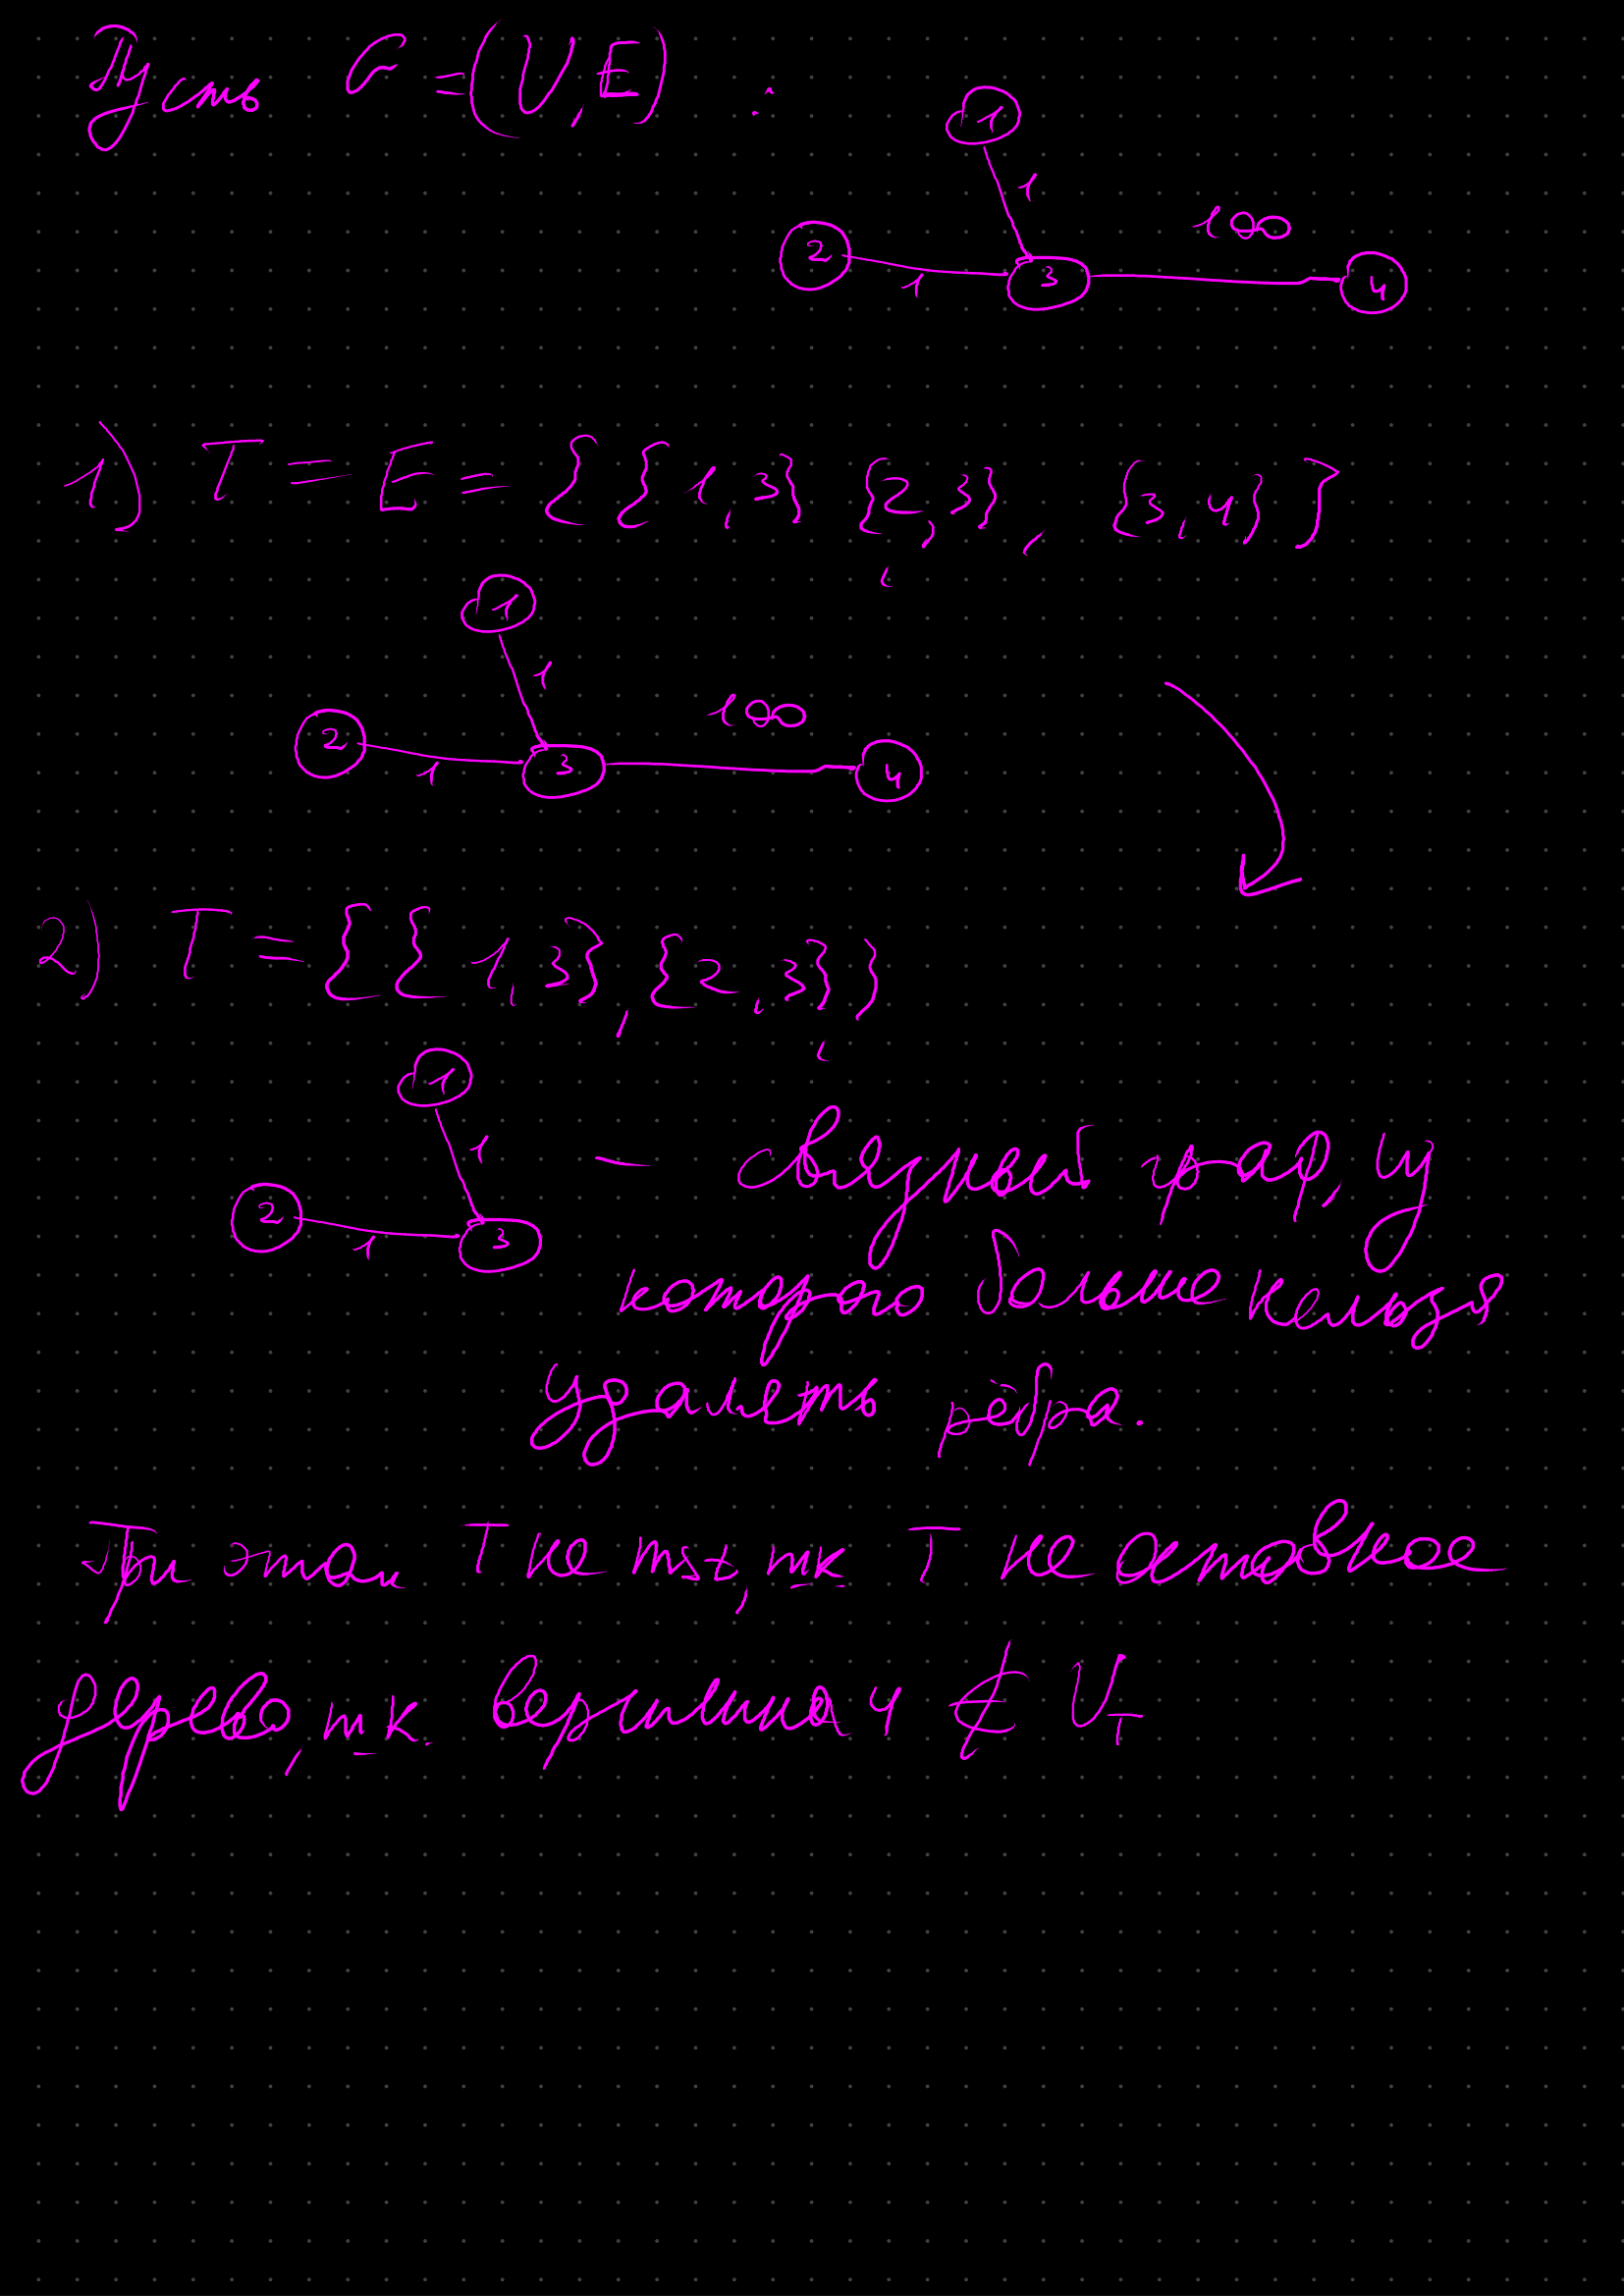
\includegraphics[scale=0.7]{a1_alg1_annotated.png}

\pagebreak

Приведём контрпример, показывающий, что алгоритм ALG\_2 не строит mst:

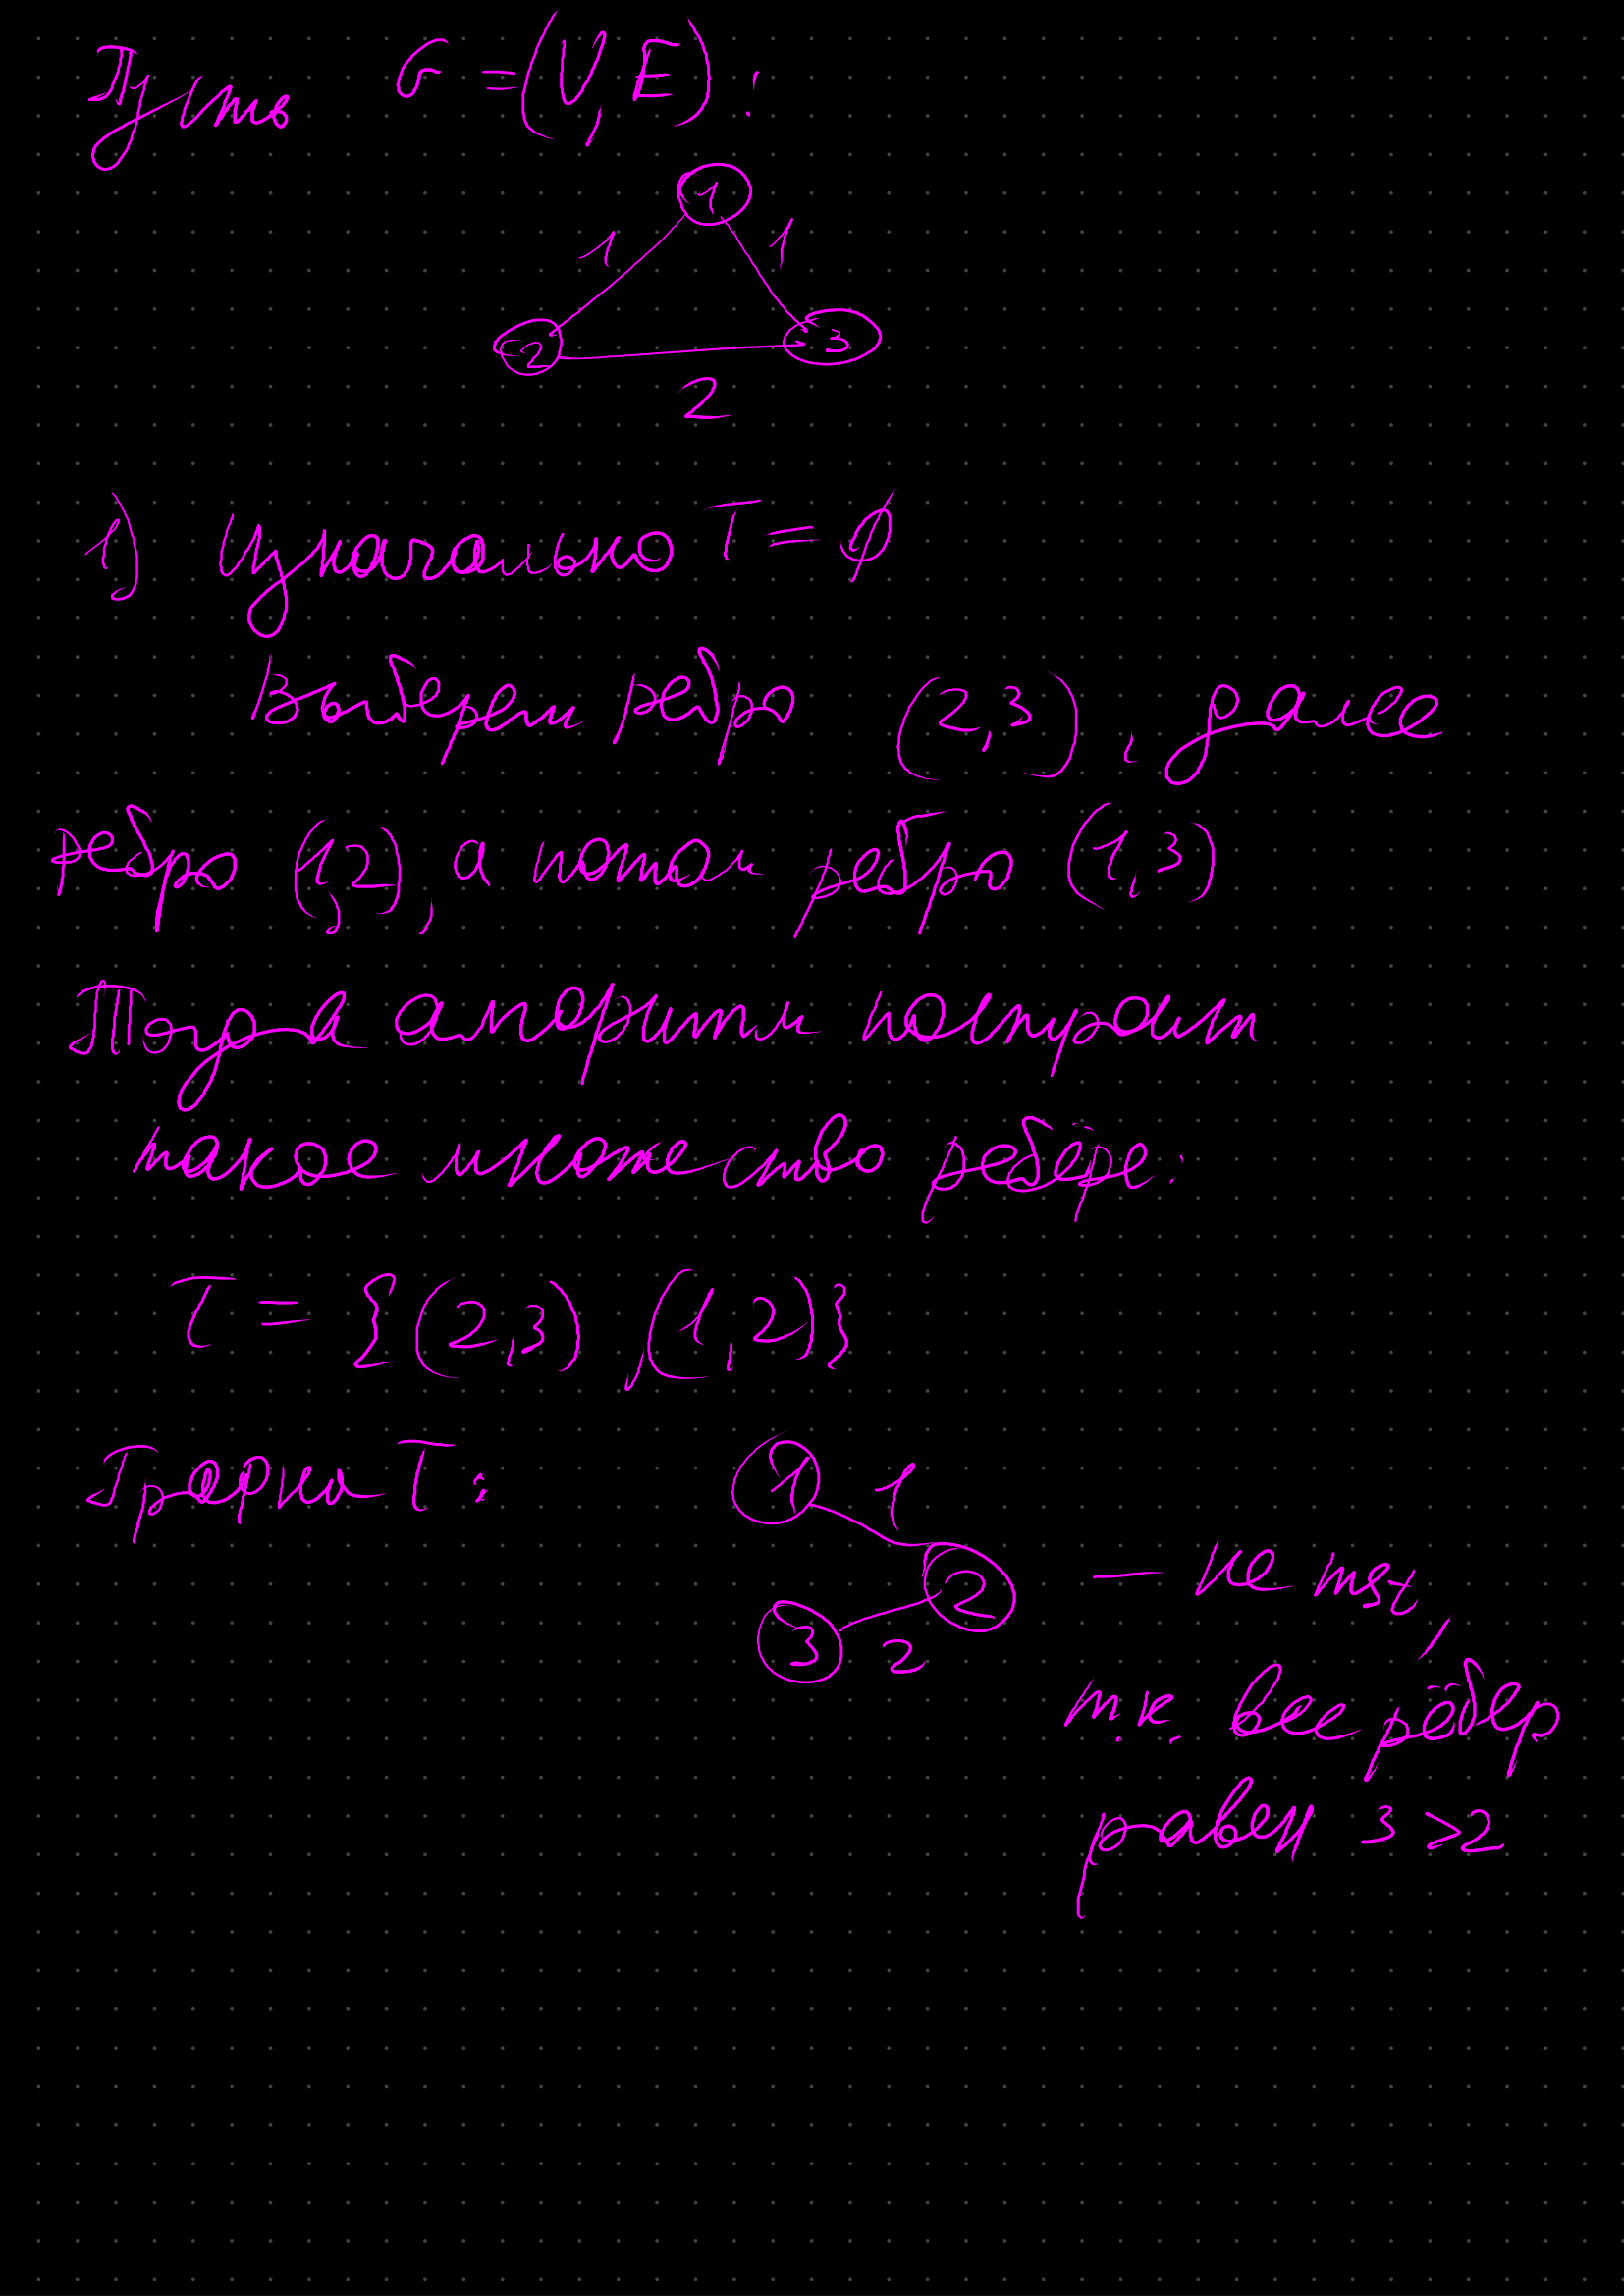
\includegraphics[scale=0.7]{a1_alg2_annotated.png}

\pagebreak

Приведём контр пример работы алгоритма ALG\_3 (построение mst):

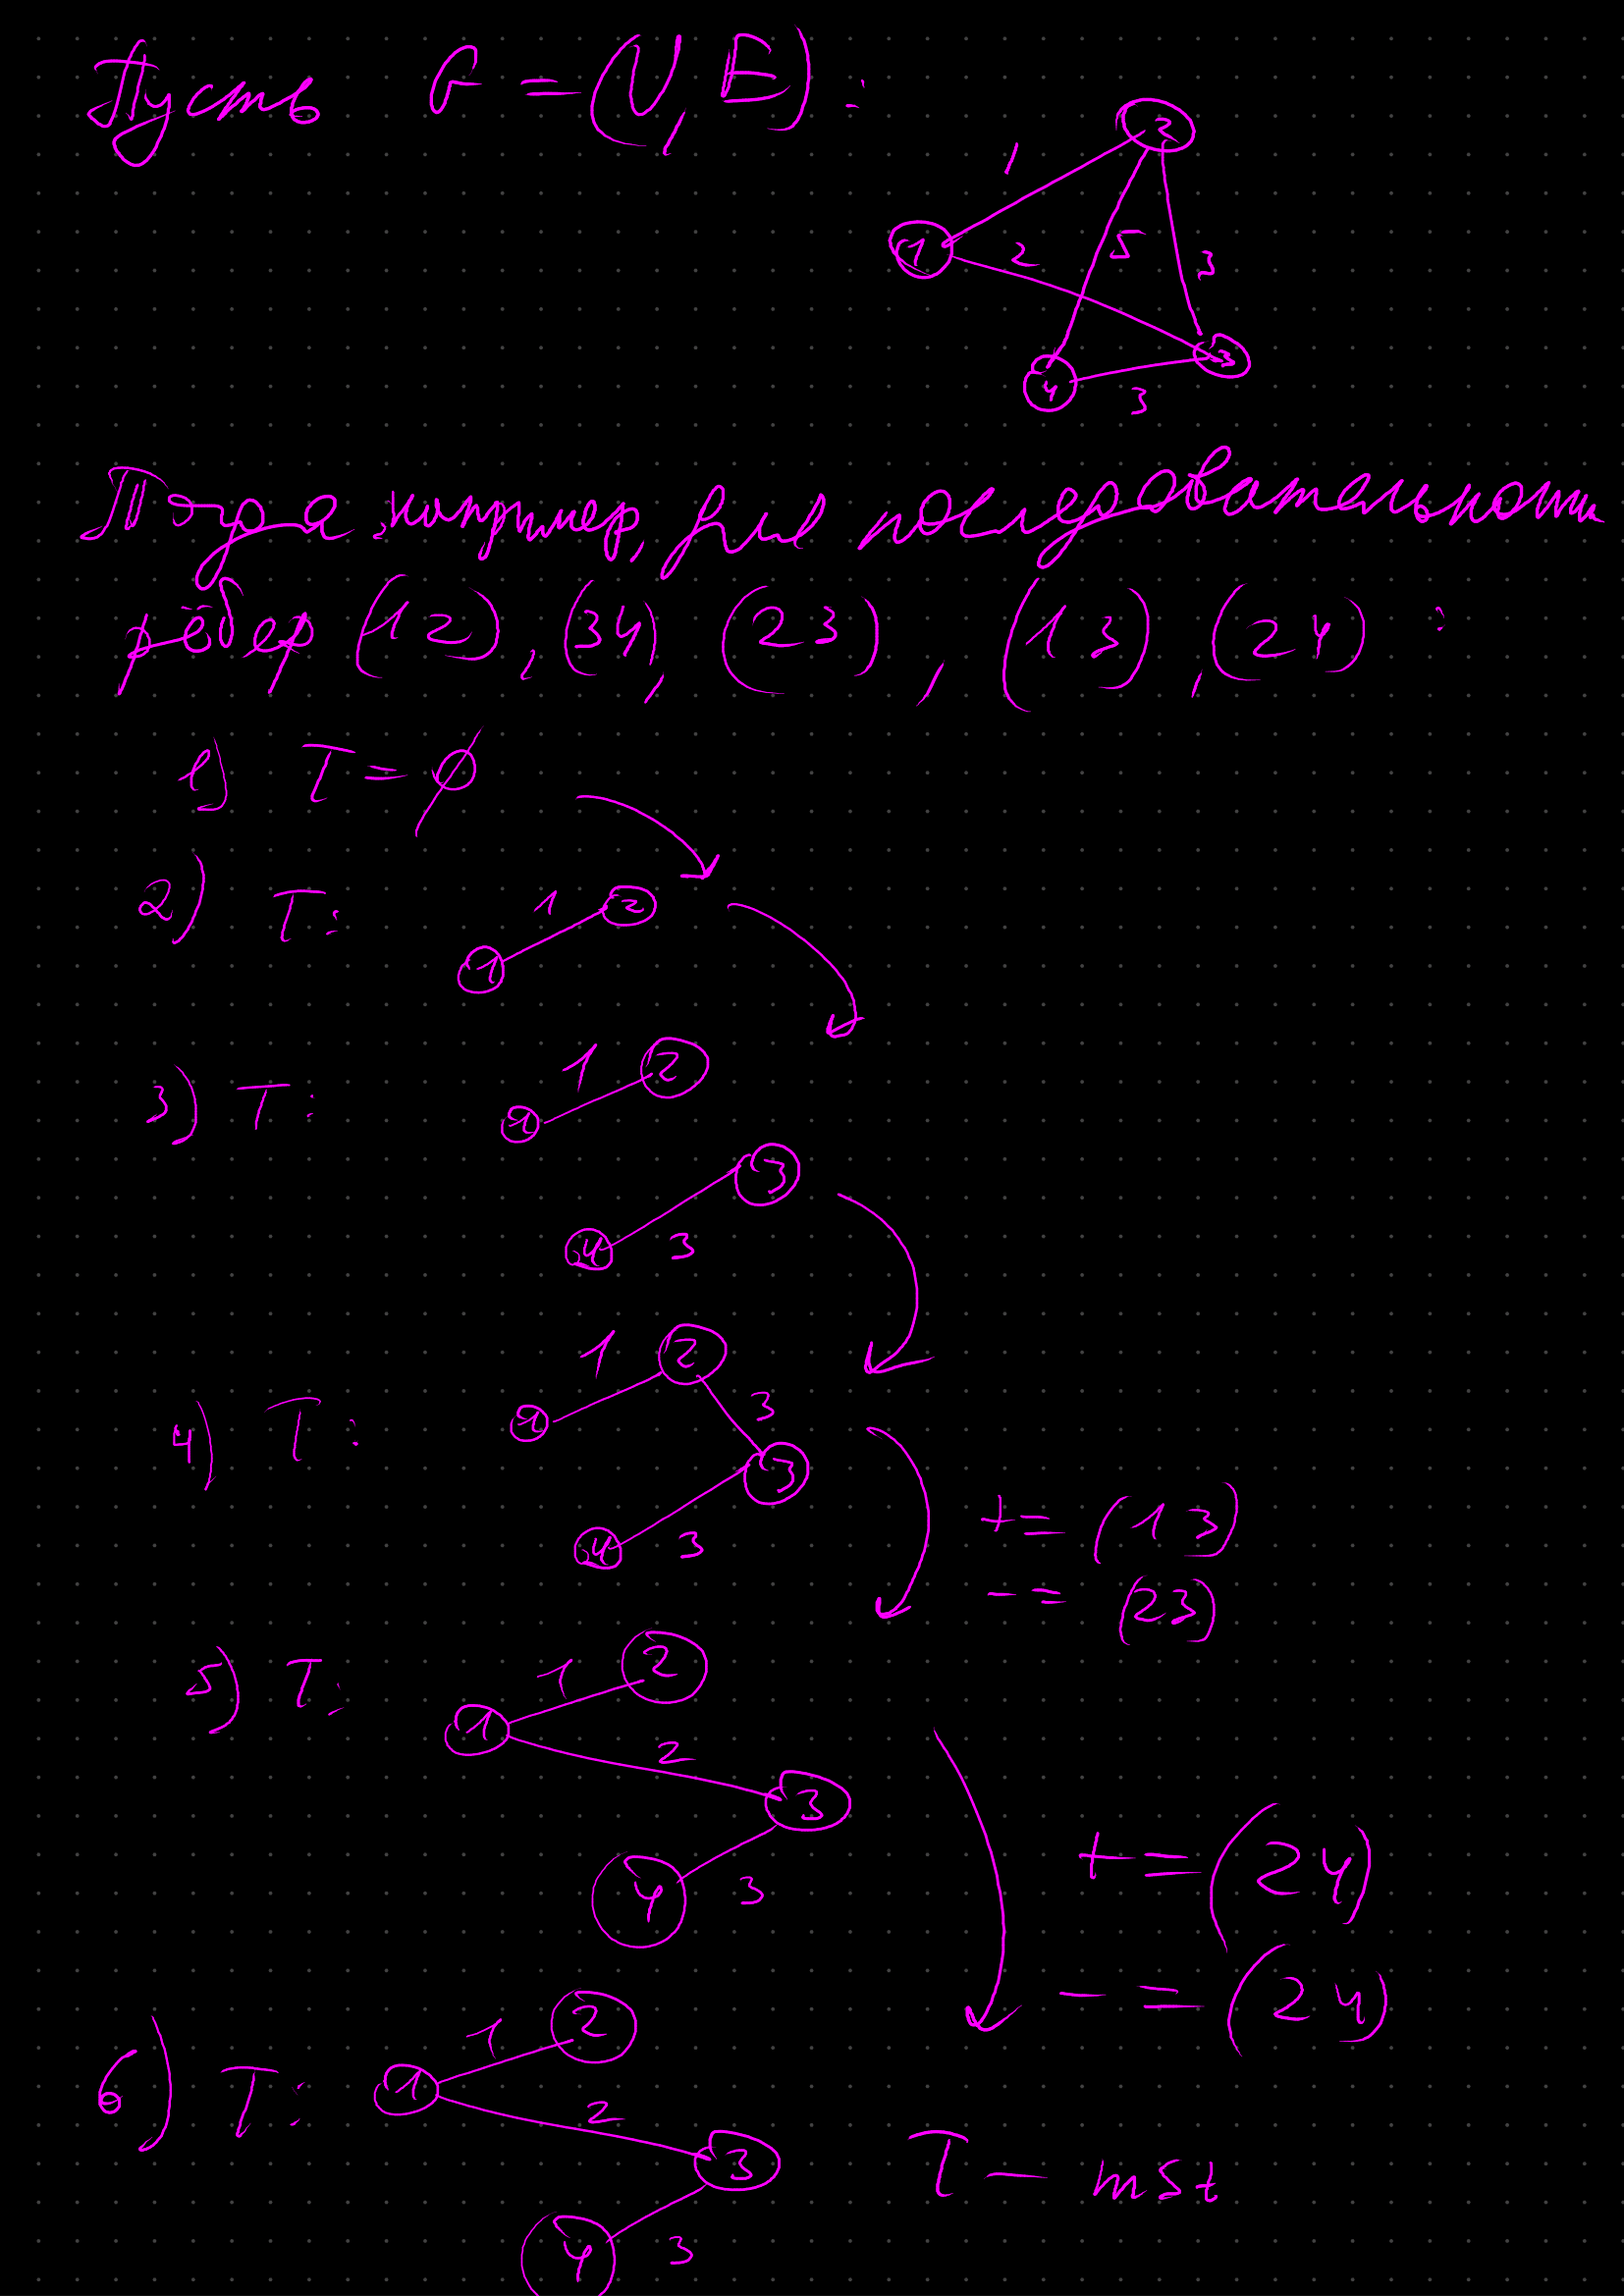
\includegraphics[scale=0.7]{a1_alg3_annotated.png}

\pagebreak

\mclemma{Лемма 1 об алгоритме ALG\_3}{
    Алгоритм ALG\_3 строит остовное дерево данного графа $ G = (V, E) $
\mcprf{
\begin{split}
    & \text{1. Здесь и далее будем обозначать черeз T граф, который построен на рёбрах,} \\
    & \text{которые получил алгоритм ALG\_3 после окончания работы.} \\
    & \text{2. До начала итераций цикла T - пустое множество, далее, на первых двух итерациях} \\
    & \text{(или одной, если $|E| = 1$) в T добавляются 2 ребра, цикл образоваться не может} \\
    & \text{3. На каждой итерации из графа T удаляется ребро $e_{max}$ после добавления} \\
    & \text{некоторого ребра $e$ тогда и только тогда, когда после добавления} \\
    & \text{ребра $e$ образовался цикл $c$, и при этом $e_{max} \in c$.} \\
    & \text{Пусть в T есть цикл. Тогда, на какой-то итерации алгоритма образовалось сразу хотя бы 2 цикла} \\
    & \text{(если на каждой итерации образовывается не более 1 цикла, то они сразу удаляются)} \\
    & \text{Рассмотрим первую среди таких итераций, на которой образовалось сразу 2 цикла.} \\
    & \text{Пусть на этой итерации было добавлено ребро $e = \{u, v\}$, тогда до добавления ребра} \\
    & \text{в графе не было циклов} \\
    & \text{(иначе, это не первая итерация, на которой появилось сразу хотя бы 2 цикла)} \\
    & \text{Т.к. на данной итерации появилось сразу хотя 2 цикла, то между вершинами} \\
    & \text{$u$ и $v$ было хотя бы 2 различных пути:} \\
    & \text{если между ними не было пути, то не образовался бы ни один цикл, а если был только один} \\
    & \text{путь, то образовался бы 1 цикл} \\
    & \text{Но раз между ними уже было хотя бы 2 различных пути, то в графе уже был цикл, что неверно,} \\
    & \text{т.е. пришли к противоречию, предположив, что в T есть цикл.} \\
    & \text{4. Т.к. в T рёбра удаляются только из циклов и только по-одному ребру, то граф связен} \\
    & \text{При этом, каждое ребро исходного графа добавлялось в T, тогда множество вершин графа T} \\
    & \text{совпадает с множеством вершин графа G (рёбра удаляются, только если они в цикле)} \\
    & \text{5. Доказали, что T - связный граф без циклов $\implies$ T - дерево.} \\
    & \text{Тогда $T = (V, E_T) \implies $ T - остовное дерево графа G.} \\
\end{split}
}
}

\mclemmaBreakable{Лемма 2 об алгоритме ALG\_3}{
    Алгоритм ALG\_3 строит минимальное остовное дерево данного графа $ G = (V, E) $
\begin{proof}
\begin{align*}
    & \text{1. По лемме 1 ALG\_3 построил некоторое остовное дерево $T = (V, E_T)$ графа G.} \\
    & \text{В данной лемме через "$mst$" будем обозначать фразу "минимальное остовное дерево"} \\
    & \text{Рассмотрим некоторые крайние случаи:} \\
    & \text{$ |V| = 0 \implies E_T = \varnothing \implies T - mst$ графа G} \\
    & \text{$ |V| = 1 \implies E_T = \varnothing \implies T - mst$ графа G} \\
    & \text{$ |V| = 2 \implies V = \{u, v\} \implies E_T = \{ \{u, v\} \} \implies T - mst$ графа G} \\
    & \text{Показали, что при $|V| \le 2$ лемма верна. Пусть $|V| > 2 \implies |V| \ge 3$} \\
    & \text{3. Граф G связен $ \implies \exists $ хотя бы одно $mst$ графа G.} \\
    & \text{Возмём произвольное $mst$ графа G, обозначив его как $T'$, и покажем, что при} \\
    & \text{помощи преобразований над рёбрами графа $T'$, которые сохраняют его свойство быть} \\
    & \text{минимальным остовным деревом графа G, из $T'$ можно получить T.} \\
    & \text{4. Если $T = T'$, то лемма доказана. Пусть $T \ne T'$.} \\
    & \text{T и $T'$ - остовные деревья графа G $ \implies |E_T| = |E_{T'}| = |V| - 1 \ge 2 $ } \\
    & T = (V, E_T) \wedge T' = (V, E_{T'}) \wedge T \ne T'
        \implies E_T \ne E_{T'} \\
    & E_T \ne E_{T'} \wedge |E_T| \ge 2 \wedge |E_{T'}| \ge 2
        \implies \exists (u, v) \in V^2: \{u, v\} \in E_{T} \wedge \{u, v\} \notin E_{T'} \\
    & \text{$T'$ - связный граф $\implies$ в графе $T'$ есть путь из вершину $u$ в вершину $v$.} \\
    & \text{Обозначим вершины этого пути как $ u, p_1, p_2, ..., p_k, v $ (быть может, k = 1)} \\
    & \text{На картинке это можно изобразить так:} \\
    & \begin{tikzpicture}
        \node[draw,align=left] at (0, 1) {В графе T:};
        \coordinate (u_T) at (0, 0);
        \coordinate (v_T) at (0, -2);
        \filldraw[black] (u_T) circle (1pt) node[anchor=south]{u};
        \filldraw[black] (v_T) circle (1pt) node[anchor=east]{v};
        \draw (u_T) -- (v_T);
        \node[draw,align=left] at (3.25, 1) {В графе $T'$:};
        \coordinate (u_TP) at (3, 0);
        \coordinate (v_TP) at (3, -2);
        \coordinate (p_1_TP) at (4, -0.2);
        \coordinate (p_k_TP) at (4, -1.8);
        \coordinate (MISSINGSENTINEL_1_TP) at (4.5, -0.6);
        \coordinate (MISSINGSENTINEL_2_TP) at (4.5, -1.4);
        \filldraw[black] (u_TP) circle (1pt) node[anchor=south]{u};
        \filldraw[black] (v_TP) circle (1pt) node[anchor=east]{v};
        \filldraw[black] (p_1_TP) circle (1pt) node[anchor=south]{$p_1$};
        \filldraw[black] (p_k_TP) circle (1pt) node[anchor=north]{$p_k$};
        \draw (u_TP) -- (p_1_TP);
        \draw[densely dotted] (p_1_TP) -- (MISSINGSENTINEL_1_TP);
        \draw[densely dotted] (MISSINGSENTINEL_2_TP) -- (p_k_TP);
        \draw (p_k_TP) -- (v_TP);
        \node [align=flush center,text width=8cm] at (1.2, -2.8) { Figure 1 };
    \end{tikzpicture} \\
    & \text{При этом, вершины } p_1, p_2, ..., p_k \in \text{ графу $T'$ }
        \implies \{ p_1, p_2, ..., p_k \} \subseteq V
        \implies \\
    & \implies \text{ эти вершины есть и в графе T (т.к. T - остовное дерево графа G)} \\
    & \text{5. Любое ребро из $E_T$ и $E_{T'}$ есть в $E \implies $ в исходном графе G есть цикл $(u, p_1, ..., p_k, v, u)$ } \\
\end{align*}
\newline
\begin{align*}
    & \text{\rom{1}. Если в графе T нет ребра $\{ v, p_k \}$, тогда:} \\
    &  \begin{tikzpicture}
        \node[draw,align=left] at (0, 1) {В графе T:};
        \coordinate (u_T) at (0, 0);
        \coordinate (v_T) at (0, -2);
        \coordinate (p_k_T) at (1, -1.8);
        \filldraw[black] (u_T) circle (1pt) node[anchor=south]{u};
        \filldraw[black] (v_T) circle (1pt) node[anchor=east]{v};
        \filldraw[black] (p_k_T) circle (1pt) node[anchor=north]{$p_k$};
        \draw (u_T) -- (v_T);
        \node[draw,align=left] at (3.25, 1) {В графе $T'$:};
        \coordinate (u_TP) at (3, 0);
        \coordinate (v_TP) at (3, -2);
        \coordinate (p_1_TP) at (4, -0.2);
        \coordinate (p_k_TP) at (4, -1.8);
        \coordinate (MISSINGSENTINEL_1_TP) at (4.5, -0.6);
        \coordinate (MISSINGSENTINEL_2_TP) at (4.5, -1.4);
        \filldraw[black] (u_TP) circle (1pt) node[anchor=south]{u};
        \filldraw[black] (v_TP) circle (1pt) node[anchor=east]{v};
        \filldraw[black] (p_1_TP) circle (1pt) node[anchor=south]{$p_1$};
        \filldraw[black] (p_k_TP) circle (1pt) node[anchor=north]{$p_k$};
        \draw (u_TP) -- (p_1_TP);
        \draw[densely dotted] (p_1_TP) -- (MISSINGSENTINEL_1_TP);
        \draw[densely dotted] (MISSINGSENTINEL_2_TP) -- (p_k_TP);
        \draw (p_k_TP) -- (v_TP);
        \node [align=flush center,text width=8cm] at (1.2, -2.8) { Figure 2 };
    \end{tikzpicture} \\
    & \text{\rom{1}.1 Ребра $ \{v, p_k\} $ нет в T $ \implies $ оно было удалено во время работы алгоритма.} \\
    & \text{Оба ребра $ \{u, v\} $ и $ \{v, p_k\} $ есть в графе G и принадлежат одному циклу, поэтому} \\
    & \text{алгоритм мог удалить любое из них, не нарушив связность T.} \\
    & \text{Из того, что алгоритм удалил $ \{v, p_k\} $, следует, что $ w(v, p_k) \ge w(u, v) $} \\
    & \text{Это верно, т.к. если $ \{v, p_k\} $ удалил из-за образования цикла после вставки $ \{u, v\}$, }\\
    & \text{то } w(v, p_k) \ge w(u, v) \\
    & \text{А если $ \{v, p_k\} $ удалили из-за другого цикла $c$, когда в графе ещё не было $\{u, v\}$, } \\
    & \text{то $w(v, p_k) \ge $ максимального веса рёбер в цикле $c$, из-за которого его удалили, но это цикл $c$ точно} \\
    & \text{проходил через вершины $ \{v, p_k\} \implies $ из-за того, что в G есть цикл $(u, p_1, ..., p_k, v, u)$, } \\
    & \text{ребро $\{u, v\}$ также попадало в цикл с рёбрами из $c$, но осталось в графе $\implies$} \\
    & \text{$\implies$ его вес не больше максимального веса рёбер в $c \implies w(u, v) \le w(v, p_k)$} \\
    & \text{\rom{1}.2 Если $ w(u, v) < w(v, p_k) $, то в $T'$ можно удалить ребро $ \{v, p_k\} $ и добавить ребро $ \{u, v\} $} \\
    & \text{Множество вершин графа $T'$ при этом не изменится, граф останется связным и в нём } \\
    & \text{не появится цикл, т.е. граф останется остовным деревом графа G.} \\
    & \text{Но при этом его (графа $T'$) вес уменьшится, что противоречит тому, что $T' - mst \implies \bot \implies$} \\
    & \text{$\implies$ предположение, что $ w(u, v) < w(v, p_k) $, неверено $ \implies w(u, v) = w(v, p_k) $} \\
    & \text{\rom{1}.3 Тогда построим граф $T''$ так: уберём из $E_{T'}$ ребро $ \{v, p_k\} $ и добавим ребро $ \{u, v\} $, т.е.} \\
    & E_{T''} := \left( E_{T'} \setminus \{ \{v, p_k\} \} \right) \cup \{ \{u, v\}  \} \text{} \\
    & \text{В графе $T''$ не появится цикл, он останется связным, и его вес не изменится, т.е. останется} \\
    & \text{равным весу графа $T' \implies T'' - mst$ графа G.} \\
    & \text{И при этом его множество рёбер $E_{T''}$ станет на 1 ребро "ближе" к множеству вершин $E_T$} \\
    & \text{Формально, } |E_{T} \cap E_{T''}| = |E_{T} \cap E_{T'}| + 1 \\
    & \text{На картинке это можно изобразить так:} \\
    &  \begin{tikzpicture}
        \node[draw,align=left] at (0, 1) {В графе T:};
        \coordinate (u_T) at (0, 0);
        \coordinate (v_T) at (0, -2);
        \coordinate (p_k_T) at (1, -1.8);
        \filldraw[black] (u_T) circle (1pt) node[anchor=south]{u};
        \filldraw[black] (v_T) circle (1pt) node[anchor=east]{v};
        \filldraw[black] (p_k_T) circle (1pt) node[anchor=north]{$p_k$};
        \draw (u_T) -- (v_T);
        \node[draw,align=left] at (3.25, 1) {В графе $T''$:};
        \coordinate (u_TS) at (3, 0);
        \coordinate (v_TS) at (3, -2);
        \coordinate (p_1_TS) at (4, -0.2);
        \coordinate (p_k_TS) at (4, -1.8);
        \coordinate (MISSINGSENTINEL_1_TS) at (4.5, -0.6);
        \coordinate (MISSINGSENTINEL_2_TS) at (4.5, -1.4);
        \filldraw[black] (u_TS) circle (1pt) node[anchor=south]{u};
        \filldraw[black] (v_TS) circle (1pt) node[anchor=east]{v};
        \filldraw[black] (p_1_TS) circle (1pt) node[anchor=south]{$p_1$};
        \filldraw[black] (p_k_TS) circle (1pt) node[anchor=north]{$p_k$};
        \draw (u_TS) -- (p_1_TS);
        \draw[densely dotted] (p_1_TS) -- (MISSINGSENTINEL_1_TS);
        \draw[densely dotted] (MISSINGSENTINEL_2_TS) -- (p_k_TS);
        \draw (u_TS) -- (v_TS);
        \node [align=flush center,text width=8cm] at (1.2, -2.8) { Figure 3 };
    \end{tikzpicture} \\
\end{align*}
\newline
\begin{align*}
    & \text{\rom{2}. Если в графе T есть ребро $\{ v, p_k \}$, тогда:} \\
    & \begin{tikzpicture}
        \node[draw,align=left] at (0, 1) {В графе T:};
        \coordinate (u_T) at (0, 0);
        \coordinate (v_T) at (0, -2);
        \coordinate (p_k_T) at (1, -1.8);
        \filldraw[black] (u_T) circle (1pt) node[anchor=south]{u};
        \filldraw[black] (v_T) circle (1pt) node[anchor=east]{v};
        \filldraw[black] (p_k_T) circle (1pt) node[anchor=north]{$p_k$};
        \draw (u_T) -- (v_T);
        \draw (p_k_T) -- (v_T);
        \node[draw,align=left] at (3.25, 1) {В графе $T'$:};
        \coordinate (u_TP) at (3, 0);
        \coordinate (v_TP) at (3, -2);
        \coordinate (p_1_TP) at (4, -0.2);
        \coordinate (p_k_TP) at (4, -1.8);
        \coordinate (MISSINGSENTINEL_1_TP) at (4.5, -0.6);
        \coordinate (MISSINGSENTINEL_2_TP) at (4.5, -1.4);
        \filldraw[black] (u_TP) circle (1pt) node[anchor=south]{u};
        \filldraw[black] (v_TP) circle (1pt) node[anchor=east]{v};
        \filldraw[black] (p_1_TP) circle (1pt) node[anchor=south]{$p_1$};
        \filldraw[black] (p_k_TP) circle (1pt) node[anchor=north]{$p_k$};
        \draw (u_TP) -- (p_1_TP);
        \draw[densely dotted] (p_1_TP) -- (MISSINGSENTINEL_1_TP);
        \draw[densely dotted] (MISSINGSENTINEL_2_TP) -- (p_k_TP);
        \draw (p_k_TP) -- (v_TP);
        \node [align=flush center,text width=8cm] at (1.2, -2.8) { Figure 4 };
    \end{tikzpicture} \\
    & \text{\rom{2}.1. Рассмотрим рёбра $\{ u, p_1 \}, ... , \{ p_k, v \}$ графа $T'$ (это множество не пусто, т.к. $k \ge 1$)} \\
    & \text{Если они все $ \in E_T $, то в $T$ есть цикл $(u, p_1, ..., p_k, v, u) \implies $ T - не дерево $ \implies \bot $} \\
    & \text{Пусть ребра $ \{p_i, p_{i+1}\} $ (здесь $0 \le i \le k - 1, p_0 := u$) нет в графе T } \\
    & \text{На картинке это можно изобразить так:} \\
    & \begin{tikzpicture}
        \node[draw,align=left] at (0, 1) {В графе T:};
        \coordinate (u_T) at (0, 0);
        \coordinate (v_T) at (0, -2);
        \coordinate (p_k_T) at (1, -1.8);
        \coordinate (p_i_T) at (1.5, -0.6);
        \coordinate (p_i_1_T) at (1.5, -1);
        \filldraw[black] (u_T) circle (1pt) node[anchor=south]{u};
        \filldraw[black] (v_T) circle (1pt) node[anchor=east]{v};
        \filldraw[black] (p_k_T) circle (1pt) node[anchor=north]{$p_k$};
        \filldraw[black] (p_i_T) circle (1pt) node[anchor=south]{$p_i$};
        \filldraw[black] (p_i_1_T) circle (1pt) node[anchor=north]{$p_{i + 1}$};
        \draw (u_T) -- (v_T);
        \draw (p_k_T) -- (v_T);
        \node[draw,align=left] at (3.25, 1) {В графе $T'$:};
        \coordinate (u_TP) at (3, 0);
        \coordinate (v_TP) at (3, -2);
        \coordinate (p_1_TP) at (4, -0.2);
        \coordinate (p_k_TP) at (4, -1.8);
        \coordinate (MISSINGSENTINEL_1_TP) at (4.5, -0.4);
        \coordinate (MISSINGSENTINEL_2_TP) at (4.5, -1.6);
        \coordinate (MISSINGSENTINEL_3_TP) at (5, -0.6);
        \coordinate (MISSINGSENTINEL_4_TP) at (5, -1.4);
        \coordinate (p_i_TP) at (5.5, -0.8);
        \coordinate (p_i_1_TP) at (5.5, -1.2);
        \filldraw[black] (u_TP) circle (1pt) node[anchor=south]{u};
        \filldraw[black] (v_TP) circle (1pt) node[anchor=east]{v};
        \filldraw[black] (p_1_TP) circle (1pt) node[anchor=south]{$p_1$};
        \filldraw[black] (p_k_TP) circle (1pt) node[anchor=north]{$p_k$};
        \filldraw[black] (p_i_TP) circle (1pt) node[anchor=south]{$p_i$};
        \filldraw[black] (p_i_1_TP) circle (1pt) node[anchor=north]{$p_{i + 1}$};
        \draw (u_TP) -- (p_1_TP);
        \draw[densely dotted] (p_1_TP) -- (MISSINGSENTINEL_1_TP);
        \draw[densely dotted] (MISSINGSENTINEL_3_TP) -- (p_i_TP);
        \draw[densely dotted] (p_i_1_TP) -- (MISSINGSENTINEL_4_TP);
        \draw[densely dotted] (MISSINGSENTINEL_2_TP) -- (p_k_TP);
        \draw (p_k_TP) -- (v_TP);
        \draw (p_i_TP) -- (p_i_1_TP);
        \node [align=flush center,text width=8cm] at (1.2, -2.8) { Figure 5 };
    \end{tikzpicture} \\
    & \text{\rom{2}.2 Ребра $ \{p_i, p_{i+1}\} $ нет в T $ \implies $ оно было удалено во время работы алгоритма.} \\
    & \text{По аналогии с пунктом \rom{1}.1 $ w(p_i, p_{i + 1}) \ge w(u, v) $} \\
    & \text{\rom{2}.3 Если $ w(u, v) < w(p_i, p_{i + 1}) $, то в $T'$ можно удалить ребро $ \{p_i, p_{i+1}\} $ и добавить ребро $ \{u, v\} $} \\
    & \text{Множество вершин графа $T'$ при этом не изменится, граф останется связным и в нём } \\
    & \text{не появится цикл, т.е. граф останется остовным деревом графа G.} \\
    & \text{Но при этом его (графа $T'$) вес уменьшится, что противоречит тому, что $T' - mst \implies \bot \implies$} \\
    & \text{$\implies$ предположение, что $ w(u, v) < w(p_i, p_{i + 1}) $, неверено $ \implies w(u, v) = w(p_i, p_{i + 1}) $} \\
    & \text{\rom{2}.4 Тогда построим граф $T''$ так: уберём из $E_{T'}$ ребро $ \{p_i, p_{i+1}\} $ и добавим ребро $ \{u, v\} $, т.е.} \\
    & E_{T''} = \left( E_{T'} \setminus \{ \{p_i, p_{i+1}\} \} \right) \cup \{ \{u, v\}  \} \text{} \\
    & \text{В графе $T''$ не появится цикл, он останется связным, и его вес не изменится, т.е. $T'' - mst$ графа G.} \\
    & \text{И при этом его множество рёбер $E_{T''}$ станет на 1 ребро "ближе" к множеству рёбер $E_T$} \\
    & \text{Формально, } |E_{T} \cap E_{T''}| = |E_{T} \cap E_{T'}| + 1 \\
\end{align*}
\newline
\begin{align*}
    & \text{На картинке это можно изобразить так:} \\
    & \begin{tikzpicture}
        \node[draw,align=left] at (0, 1) {В графе T:};
        \coordinate (u_T) at (0, 0);
        \coordinate (v_T) at (0, -2);
        \coordinate (p_k_T) at (1, -1.8);
        \coordinate (p_i_T) at (1.5, -0.6);
        \coordinate (p_i_1_T) at (1.5, -1);
        \filldraw[black] (u_T) circle (1pt) node[anchor=south]{u};
        \filldraw[black] (v_T) circle (1pt) node[anchor=east]{v};
        \filldraw[black] (p_k_T) circle (1pt) node[anchor=north]{$p_k$};
        \filldraw[black] (p_i_T) circle (1pt) node[anchor=south]{$p_i$};
        \filldraw[black] (p_i_1_T) circle (1pt) node[anchor=north]{$p_{i + 1}$};
        \draw (u_T) -- (v_T);
        \draw (p_k_T) -- (v_T);
        \node[draw,align=left] at (3.25, 1) {В графе $T''$:};
        \coordinate (u_TS) at (3, 0);
        \coordinate (v_TS) at (3, -2);
        \coordinate (p_1_TS) at (4, -0.2);
        \coordinate (p_k_TS) at (4, -1.8);
        \coordinate (MISSINGSENTINEL_1_TS) at (4.5, -0.4);
        \coordinate (MISSINGSENTINEL_2_TS) at (4.5, -1.6);
        \coordinate (MISSINGSENTINEL_3_TS) at (5, -0.6);
        \coordinate (MISSINGSENTINEL_4_TS) at (5, -1.4);
        \coordinate (p_i_TS) at (5.5, -0.8);
        \coordinate (p_i_1_TS) at (5.5, -1.2);
        \filldraw[black] (u_TS) circle (1pt) node[anchor=south]{u};
        \filldraw[black] (v_TS) circle (1pt) node[anchor=east]{v};
        \filldraw[black] (p_1_TS) circle (1pt) node[anchor=south]{$p_1$};
        \filldraw[black] (p_k_TS) circle (1pt) node[anchor=north]{$p_k$};
        \filldraw[black] (p_i_TS) circle (1pt) node[anchor=south]{$p_i$};
        \filldraw[black] (p_i_1_TS) circle (1pt) node[anchor=north]{$p_{i + 1}$};
        \draw (u_TS) -- (p_1_TS);
        \draw[densely dotted] (p_1_TS) -- (MISSINGSENTINEL_1_TS);
        \draw[densely dotted] (MISSINGSENTINEL_3_TS) -- (p_i_TS);
        \draw[densely dotted] (p_i_1_TS) -- (MISSINGSENTINEL_4_TS);
        \draw[densely dotted] (MISSINGSENTINEL_2_TS) -- (p_k_TS);
        \draw (p_k_TS) -- (v_TS);
        \draw (u_TS) -- (v_TS);
        \node [align=flush center,text width=8cm] at (1.2, -2.8) { Figure 6 };
    \end{tikzpicture} \\
    & \text{6. Таким образом, привели пример итерационного алгоритма, который на каждой итерации} \\
    & \text{преобразует $mst T^{j}$ в $mst T^{j + 1}$ путём удаления одного ребра из $E_{T^j}$ и добавления} \\
    & \text{одного ребра из $E_T$, которого ранее не было в $E_{T^j}$, так, что множества вершин графов $T^j$ и $T^{j + 1}$} \\
    & \text{совпадают и равны $V$, и при этом выполняется равенство $ |E_T \cap E_{T^{j + 1}} | = |E_T \cap E_{T^{j}} | + 1 $ } \\
    & \forall j: | E_{T^j} | = |V| - 1 \implies \forall j: |E_T \cap E_{T^{j}} | \le |V| - 1 \\
    & \text{Тогда через конечное число итераций алгоритма получим $mst T^l$, такое что: } |E_T \cap E_{T^{l}} | = |V| - 1 \\
    & \left(|E_T| = |V| - 1\right)
        \wedge \left(|E_{T^l}| = |V| - 1\right)
        \wedge \left(|E_T \cap E_{T^{l}} | = |V| - 1\right)
        \implies E_T = E_{T^l} \\
    & \text{У графов $T$ и $T^l$ множества вершин совпадают $\implies T = T^l$} \\
    & \text{Таким образом, через конечное число итераций получим $mst T^l$, равное T $ \implies T - mst$ графа G} \\
\end{align*}
\end{proof}
}

\end{document}
